% !TeX root = ../main.tex
% HLD: high level design


\chapter{概要设计}

本文需求分析章节的内容对本中文时间表达式信息抽取系统进行了详尽的需求分析,明晰了该中文时间表达式信息抽取系统需要实现的功能及其他的性能要求。
本章节将基于在第三章中分析所得的功能性需求和非功能性需求,对本中文时间表达式信息抽取系统进行概要设计,并且对该中文时间表达式信息抽取系统的整体架构以及各个模块的功能设计进行详细阐述。
通过该章节的工作内容,读者可以从总体上了解整个系统的设计思路。
本章节的工作为后续详细设计与实现做准备.

\section{系统整体架构设计}

由于笔者所在企业的开发要求, 软件系统的整体体系架构采用的是浏览器-服务器体系结构, 即B/S(Browser/Server)架构, 通过基于B/S架构的SaaS(Soft as a Service)平台向用户提供服务.
其中浏览器界面负责与客户的信息交互, 在运行时间表达式的识别和解析之前, 负责获取用户输入的语料和相关的配置等.
服务器后端开发则采用的是典型的四层架构模式, 分别为用户接口(API, Application Programming Interface)层, 外观(Facade)模式层, 服务(Service)层, 数据访问(DAO, Data Access Object)层. 详情见下图.

用户接口层是服务器端与浏览器或其他形式的数据传输方式的第一站, 用户接口层不做过于复杂的逻辑处理, 只是将系统内部提供给用户的功能暴露在外, 方便与用户交互或被开发人员调用.
在用户接口层承接网络中传入的数据, 并将其用系统内部的数据结构封装, 传递给外观模式层.

外观模式层是整个服务器后端的业务逻辑核心, 可以被认为是业务逻辑层. 外观模式获取到用户接口封装的数据结构并将其解包.
由之前的需求分析可知, 用户可能通过用户界面传入单条语句或者多条语句对中文时间表达式信息抽取系统做可行性的检验, 观察系统的输出结果,
也可能传入容量较大的文档, 或者图片以及PDF文档. 这时需要使用辅助的OCR模块对用户输入做相应的处理. 将非文字的形式转变为系统可以接受的字符串形式.
在解包用户输入以及对用户输入做预处理后, 这些数据将被中文时间表达式识别模块接收.
中文时间表达式模块会根据底层的基本元素组合出规则, 通过规则匹配的形式将中文时间表达式这一类实体从起来源的语料中提取出来, 然后将其抽象化为特殊的元素形式, 最后将这些元素提交给中文时间表达式解析模块.
中文时间表达式解析模块将识别模块识别出的元素作为叶结点, 自下而上的构建出一棵或多棵语法树, 当出现多棵语法树时, 将通过朴素贝叶斯选择器模块进行辅助, 判断决策采用哪一棵树作为最终生成的结果树.
结果树在解析的过程中会被自然的携带结构化的时间信息, 最终在根结点可以直接格式化为UTC形式的时间.

服务层主要负责和数据库交互的服务逻辑, 负责将外观模式层的处理结果最终保存到数据库中进行持久化.
如果没有服务层作为数据库与业务逻辑之间的桥梁, 那大量有价值的原始语料或解析结果将不复存在.
服务层会对数据库中的操作进行简单的聚合, 完成较为复杂的数据存取操作.

数据访问层是对数据库表中行记录的具现化, 是对象关系映射模型(ORM, Object Relation Mapping)的具体实现, 数据访问层详细的表示了数据库中存储的行记录中各个字段或属性的名称以及类型.
为服务层针对数据库表的操作提供了一定的便捷性.

此外, 为了方便用户进行批处理, 即传入大量的文档或图片. 本中文时间表达式信息抽取系统采用分布式的方法来优化批处理任务.
系统内部一共部署了六台逻辑服务器, 其中三台运行中文时间表达式信息抽取系统, 用作任务服务器, 一台服务器专做数据库服务器, 以存储中间数据, 一台服务器作为静态资源服务器, 一台服务器作为反向代理服务器.
三台任务服务器都使用多线程的方式运行中文时间表达式信息抽取系统, 而代理服务器采用复杂均衡的方式将用户请求产生的负载较为均匀的分配在三台任务服务器上. 复杂均衡的分布式运算使得批处理的时间大大剪短.
中文时间表达式信息抽取系统的网络拓扑图如下图所示.


\section{系统功能模块设计}

在制作中文时间表达式信息抽取系统的功能结构善主要参照的原则是:
在模块的内部高度集聚,每个模块之间的连接性不高的原则,和固有的制作软件的要求一样,将相互管理
的模块进行合并,然后对相互的数据进行转换.
在系统内部,并未划分一个独立的方面来进行数据的交流转换,在这样的区别之后,能够更加方便的完成吸引的功能,按照每个方面彼此之间的关联,可以使各个子系统分层次的进行制作和开发,使用调用的形式来完成每个模块的要求。
利用系统整体架构设计中提到的用户接口层、外观模式层、服务层, 数据访问层四者者之间的联系来对子系统进行划分。
在单独制作模块的过程中,使用单独的制作来完成功能,确保每个用户功能的单独性,不会因为极小的变动就会影响全局,使系统的更新和改善互相独立,使系统更加的安全。
使用模块的划分来展示系统的作用来进行相应的开发。







\begin{figure}[h]
  \centering
  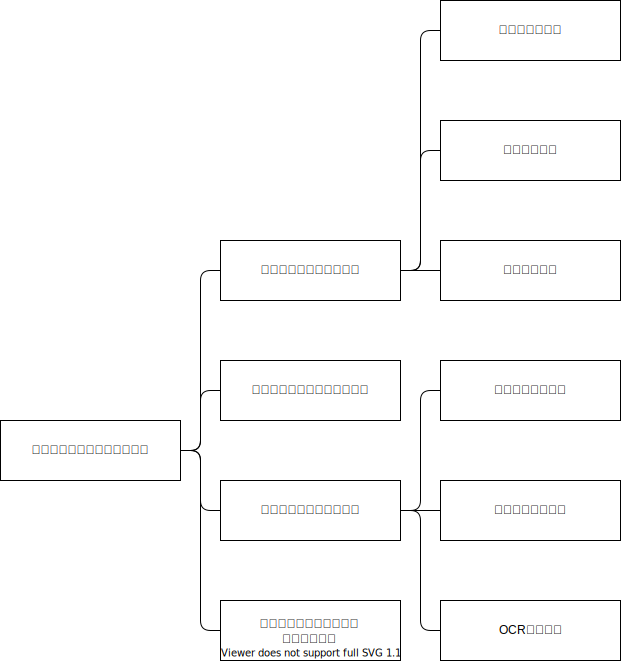
\includegraphics[width=1\textwidth]{系统功能模块.pdf}
  \caption{系统功能模块图}
  \label{fig:badge}
\end{figure}



